\chapter{Applications of TDA}
\graphicspath{ {/home/tomasp/Dokumenty/Master_Thesis/figures/} }

In this section, we will go over some of the more popular methods, techniques and algorithms that are used within Topological Data Analysis. The most theoretically demanding one is Persistent Homology that we worked on introducing in the previous chapters in the most basic and stripped down manner to not overwhelm the reader. We will look at the popular clustering and dimensionality reducing algorithms such as UMAP and Mapper, both closely related to each other. In the direction of homology, we will look at other equivalent and potentially more useful representations such as persistence images, landscapes and entropy. We will demonstrate them on the classical setting of point clouds but also time series and graphs.

All methods will be accompanied by examples, both toy examples to better understand and real-life data to show one can use the methods to obtain new information. It is hopelessly naive to believe that we can summarize all the ways TDA and its surrounding methods have been and can be used to. As such, the reader will be pointed to different articles that cover more intricate applications that go beyond the scope of this work.

\section{UMAP}
UMAP, short for \textit{Uniform Manifold Approximation and Projection for Dimension Reduction}, is a dimension reduction technique, similar to something like t-SNE, that is commonly used for dataset visualization, clustering, filtering or embedding within neural networks. UMAP and Mapper complement each other and are usually used together, hence why we talk about UMAP first.

UMAP is built on three, relatively reasonable, assumptions about your dataset:
\begin{itemize}
  \item The data is uniformly distributed on a Riemannian manifold.
  \item The Riemannian metric is locally constant or can be approximated as such.
  \item The Riemannian manifold is locally connected.
\end{itemize}

If the assumptions are satisfied, it is then possible to model the ambient manifold with what we call a \textit{fuzzy} topological structure. We will briefly explain and summarize the workings of the algorithm, although it is recommended to read the original article \cite{mcinnes2020umapuniformmanifoldapproximation} for a more detailed explanation.

The first step is to approximate the manifold the data supposedly lies on. Assuming that the manifold isn't known in advance (perhaps from some theoretical description of the model), we need to approximate the geodesic distance. It simplifies the problem to assume that the data is uniformly distributed on the manifold. Given this, we can center balls of an appropriate radius around each point to obtain a crude approximation of the manifold. We can then approximate geodesic distances from each ball to its neighbour.

Unfortunately, this means that we have independent notions of distances that may or may not be compatible. To merge all the local metric spaces into one compatible global structure, we utilize fuzzy simplicial sets, where a fuzzy set is characterized by a carrier set $A$ and a map $\mu: A \to [0,1]$ we call the membership function. This turns membership from a property attaining two values -- true or false -- into a property taking values in the unit interval. Each metric space is translated into a fuzzy simplicial set via a categorical construction (the fuzzy singular set functor).

The goal, once we have constructed our fuzzy simplicial set, is to find a low-dimensional representation of our data that closely matches the topological structure. This optimal embedding is found after minimizing the error between the two representations with respect to cross entropy of the fuzzy sets. From a purely computational perspective, UMAP can be described in terms of weighted graphs; placing UMAP in the class of graph learning algorithms such as Isomap, the above-mentioned t-SNE and Laplacian Eigenmaps.

We will go over some examples of UMAP on well-known datasets and later compare the obtained results with the one we will see with Mapper in the next section.

\subsection{Penguin dataset}
We will start with a simple example using the known Penguin dataset \cite{10.1371/journal.pone.0090081}. The simplicity of the dataset will make it easier to highlight and interpret the results from UMAP. The dataset has few features, as seen in \ref{tab:penguins}, with some data missing and replaced with NaNs. While it would be recommended to use some form of imputation to replace them in a proper study, we will simply drop the missing values in this example without worrying too much.

The dataset itself contains measurements about bill dimensions and flipper lengths, alongside metadata regarding the penguin's body mass and sex. The values we will focus on are the first four, ignoring the species and island variables. There are a total of 333 penguins in this dataset, and we can start with a simple pairwise scatter plot matrix to get a rough idea of what we're dealing with, seen in \ref{fig:penguins_scatter}

\begin{table}[]
\centering
\resizebox{\textwidth}{!}{%
\begin{tabular}{|c|c|c|c|c|c|c|c|c|}
\hline
 &
  \textbf{species} &
  \textbf{island} &
  \textbf{bill\_length\_mm} &
  \textbf{bill\_depth\_mm} &
  \textbf{flipper\_length\_mm} &
  \textbf{body\_mass\_g} &
  \textbf{sex} &
  \textbf{year} \\ \hline
0 & Adelie & Torgersen & 39.1 & 18.7 & 181.0 & 3750.0 & male   & 2007 \\ \hline
1 & Adelie & Torgersen & 39.5 & 17.4 & 186.0 & 3800.0 & female & 2007 \\ \hline
2 & Adelie & Torgersen & 40.3 & 18.0 & 195.0 & 3250.0 & female & 2007 \\ \hline
3 & Adelie & Torgersen & NaN  & NaN  & NaN   & NaN    & NaN    & 2007 \\ \hline
4 & Adelie & Torgersen & 36.7 & 19.3 & 193.0 & 3450.0 & female & 2007 \\ \hline
\end{tabular}%
}
\caption{First five rows of the Penguin dataset.}
\label{tab:penguins}
\end{table}

\begin{figure}[h!]
  \centering
  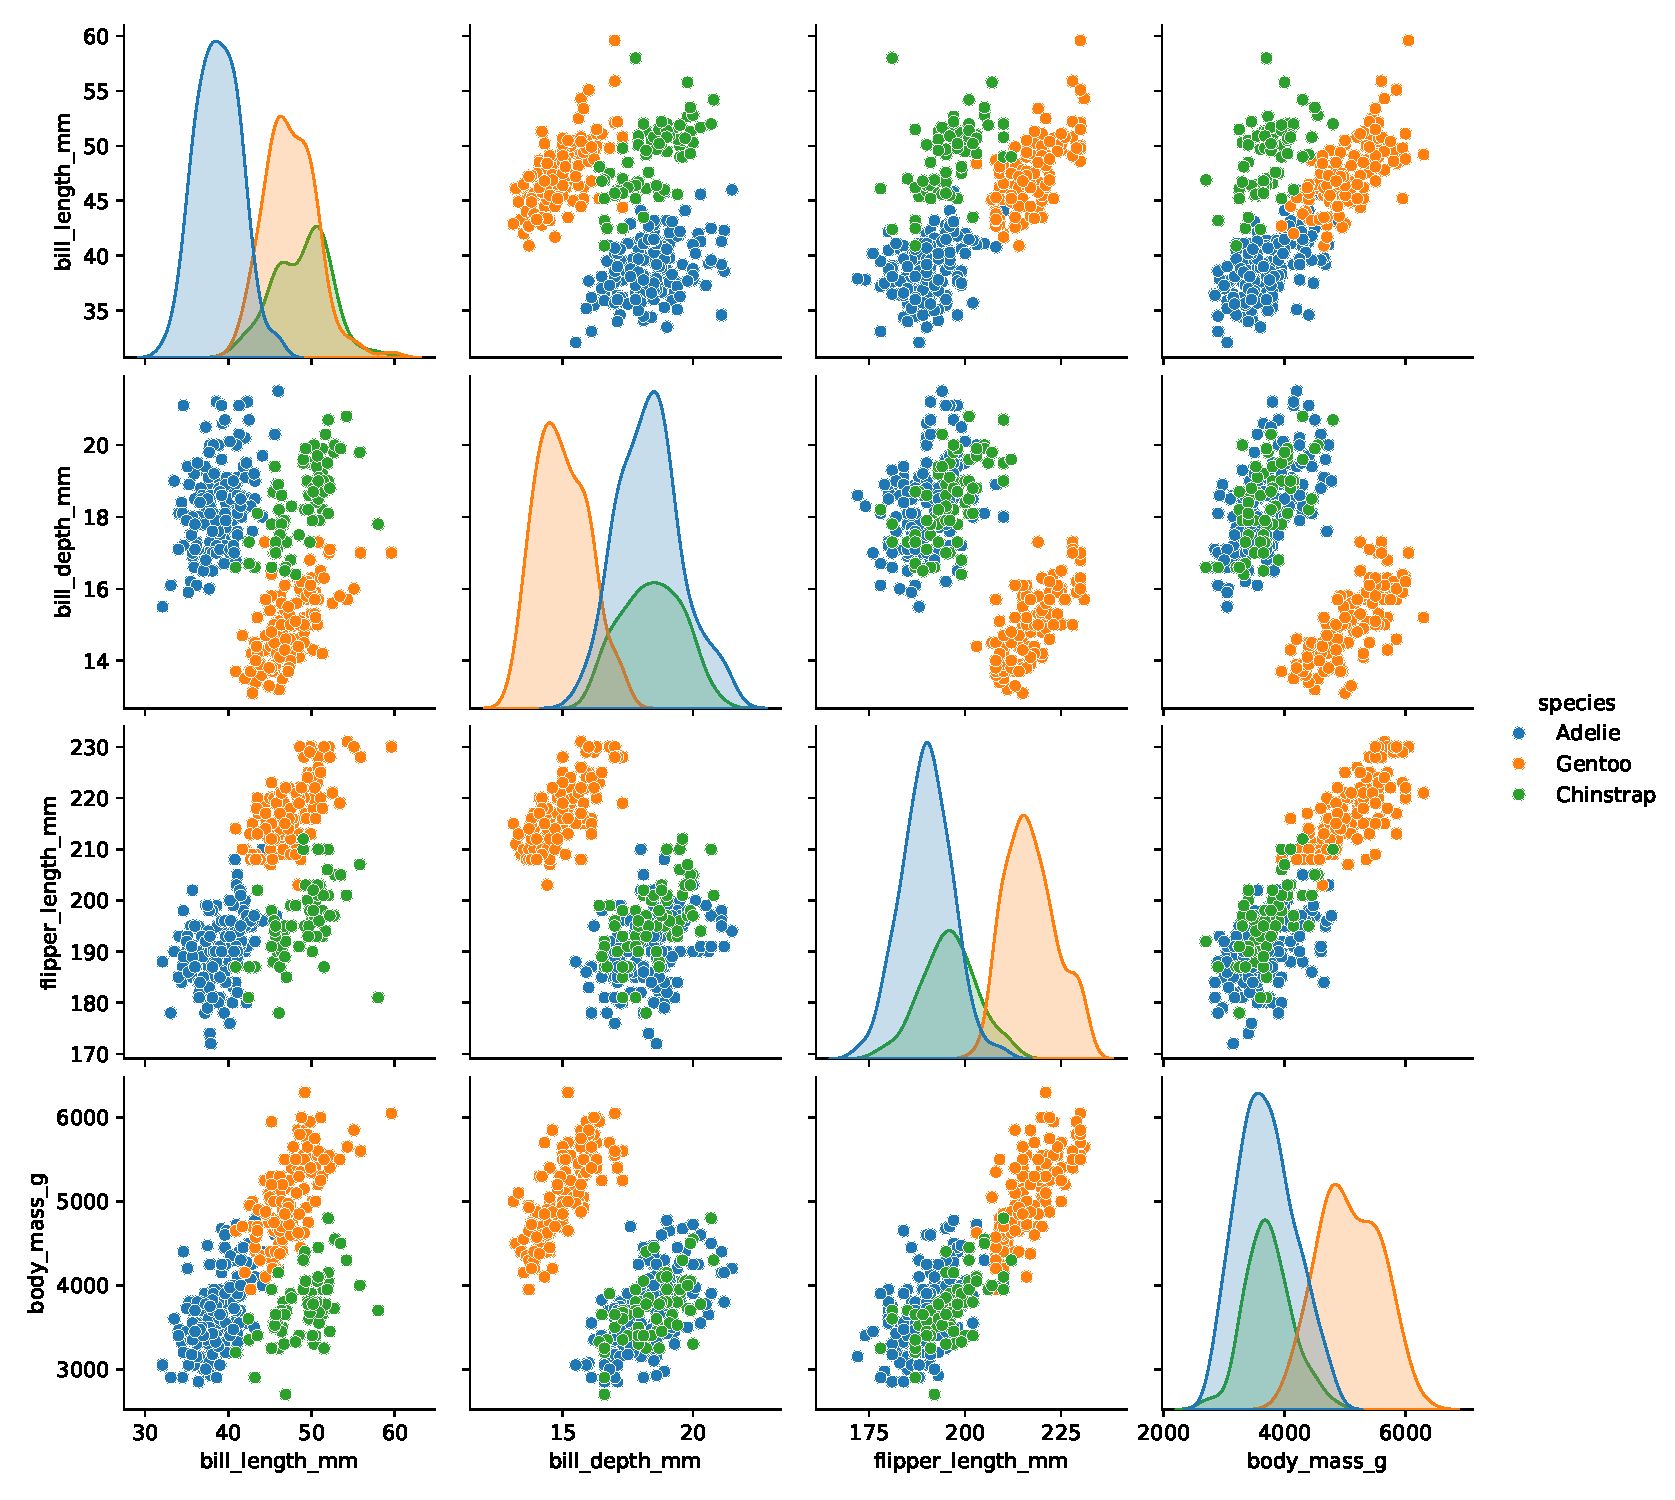
\includegraphics[width=15cm, height=13.5cm]{Penguins_scatterplot.pdf}
  \caption{Pairwise plots of the Penguin dataset for the bill length, bill depth, flipper length and body mass variables.}
  \label{fig:penguins_scatter}
\end{figure}

For this task, we will use the Python library UMAP \cite{mcinnes2018umap-software} to reduce the dimension in a way that preserves the topology of the 4-dimensional space we are working with. We can first remove the missing values and the columns we won't need for this short analysis. Since we are working with different scales, it is generally useful to convert the features into z-scores or use a different scaler process.

\begin{figure}[h!]
  \centering
  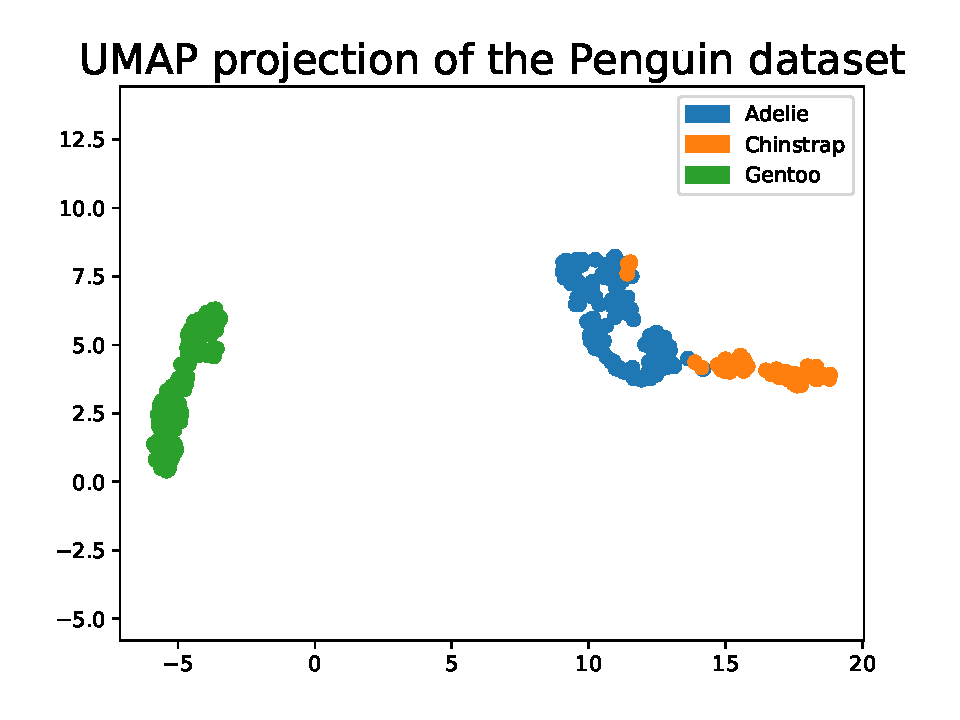
\includegraphics[width=12cm, height=10cm]{penguins_projection.pdf}
  \caption{UMAP dimension reduction result on the Penguin dataset.}
  \label{fig:penguins_projection}
\end{figure}

The result of reducing the dimension can be seen in \ref{fig:penguins_projection}. Comparing it to \ref{fig:penguins_scatter}, it does a good job of capturing the relationships between the three groups. Although, in this case specifically, we already found everything we needed in the scatter plot matrix, which was only possible because we worked with four dimensions. Once the number of features is higher, a scatter plot matrix becomes unwieldy and difficult to read properly.

\subsection{Digits dataset}
For an example with a high number of features, we can consider the known digits dataset \cite{optical_recognition_of_handwritten_digits_80}, one of the many toy datasets used to validate both old and new algorithms. We can iterate over the individual images to display them on a grid in \ref{fig:digits} to see what we are working with.

\begin{figure}[h!]
  \centering
  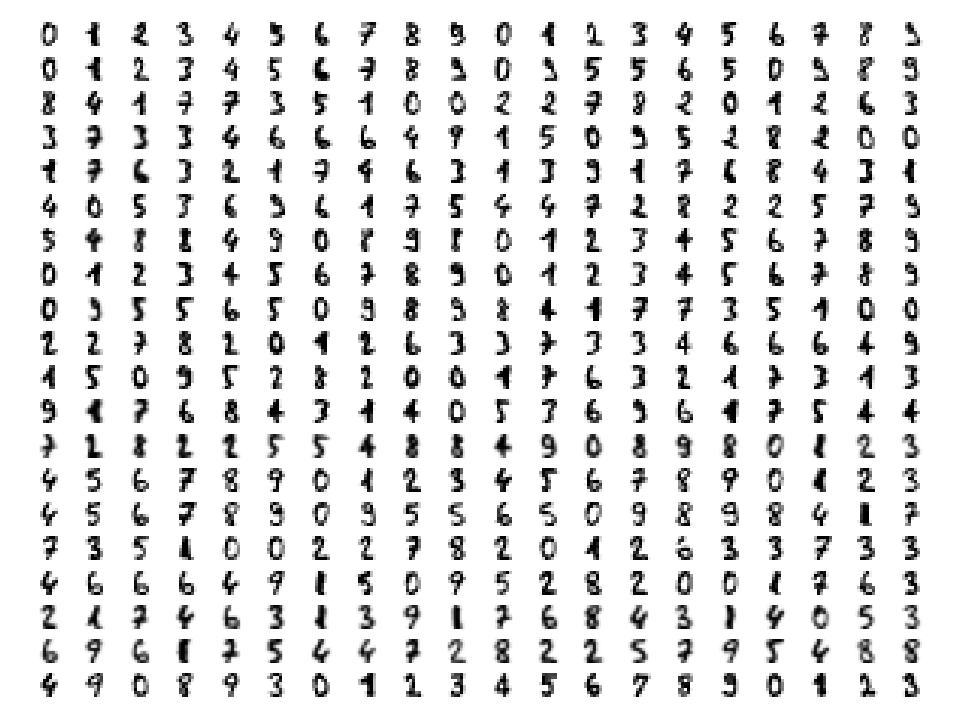
\includegraphics[width=12cm, height=10cm]{digits.pdf}
  \caption{First few images of the digits dataset}
  \label{fig:digits}
\end{figure}

The digits dataset contains 1797 bitmaps of hand-written digits in 10 classes -- each class corresponding to its digit. Most digits are somewhat readable but there are few that are simply too blurred to be considered useful. Such bitmaps should be separated into their own cluster of outliers, creating one additional class in the end.
The usual goal is to classify and cluster each bitmap into its appropriate class. We will see that with UMAP, we obtain satisfying results with a simple application of the algorithm.
